\documentclass[12pt,a4paper]{article}

% 如果需要中文支持,推荐使用xeCJK + 字体设置
\usepackage{xeCJK}
\setCJKmainfont{SimSun}  % 示例:宋体,可根据系统字体情况更换
\usepackage{amsmath}      % 数学公式(如有需要)
\usepackage{graphicx}     % 插图
\usepackage{geometry}     % 调整页边距
\usepackage{fancyhdr}     % 自定义页眉页脚
\usepackage{indentfirst}  % 中文首行缩进
\usepackage{calc}         % 允许做长度运算(测量文字宽度等)
\usepackage{titlesec}
\usepackage{booktabs} % 解决 \midrule 和 \bottomrule 报错
\usepackage{enumitem} % 支持自定义列表格式
\usepackage{float}

% 设置 \section 级标题为:加粗、大字号(如 \Large)
\titleformat{\section}
	{\bfseries\large}    % 标题自身的格式
	{\thesection}        % 标题编号的显示方式
	{1em}                % 编号与标题文字之间的间距
	{}                   % 在标题文字前后可插入额外代码,此处为空
	
% 设置 \subsection 级标题为:加粗、中等字号(如 \normalsize)
\titleformat{\subsection}
	{\bfseries\normalsize}
	{\thesubsection}
	{1em}
{}

% 页面设置(可根据需要微调)
\geometry{
	left=2cm,
	right=2cm,
	top=1cm,
	bottom=1.5cm
}

% 不需要过大的行距,使用较接近单倍行距的设置
\renewcommand{\baselinestretch}{1}

% 仅在页脚居中显示页码,页眉保持为空
\pagestyle{fancy}
\fancyhf{}  % 清空默认的页眉页脚
\fancyfoot[C]{\thepage}
\renewcommand{\headrulewidth}{0pt}
\renewcommand{\footrulewidth}{0pt}

% 首行缩进2字符(中文习惯)
\setlength{\parindent}{0pt}
\setlength{\leftskip}{2em}

\begin{document}
	%-------------------------------------------------------
	% 1 并排两个minipage:左标题、右校徽
	%   - 0.65\textwidth + 0.35\textwidth = \textwidth
	%   - 如果校徽过大或过小,可改宽度,如 0.25\textwidth、0.3\textwidth 等
	%   - 如果想让标题更大,可将 \Huge 改成 \huge 或 \LARGE
	%-------------------------------------------------------
	\noindent
	\hspace{-2em}
	\begin{minipage}[c]{0.65\textwidth}
		\raggedright
		{\fontsize{40pt}{60pt}\selectfont 物理实验报告}
	\end{minipage}
	\begin{minipage}[c]{0.35\textwidth}
		\raggedleft
		% 强制把校徽拉大到 0.35\textwidth 宽度 (高度自动匹配)
		% 若想指定高度,可用 "height=3cm" 等. 二选一即可.
		
\includegraphics[width=\linewidth, trim={20cm 20cm 20cm 20cm}, clip]{university_logo.png}
	\end{minipage}

	\vspace{-1em}
	

	%下方画两条分割线,并在两线之间写学号、姓名、日期、时间
	
	\hrule
	\vspace{0.4em}
	\noindent
	\begin{tabular}{l l l l}
    学号:\underline{12411415} & 姓名:\underline{左嘉宇} &
    日期:\underline{2025/03/25} & 时间:\underline{周二下午}
	\end{tabular}
	\vspace{-0em}
	\par
	\hrule

	





	%正文示例

	
	\section{实验名称:声速测量}
	
	\section{实验目的}
		了解压电换能器工作原理,学习超声波的产生、发射和接收\\
		分别使用驻波法和相位法测量波长和声速

	\section{实验仪器}
		信号发生器、示波器、超声声速测定仪
		\begin{figure}[H]
			\centering
			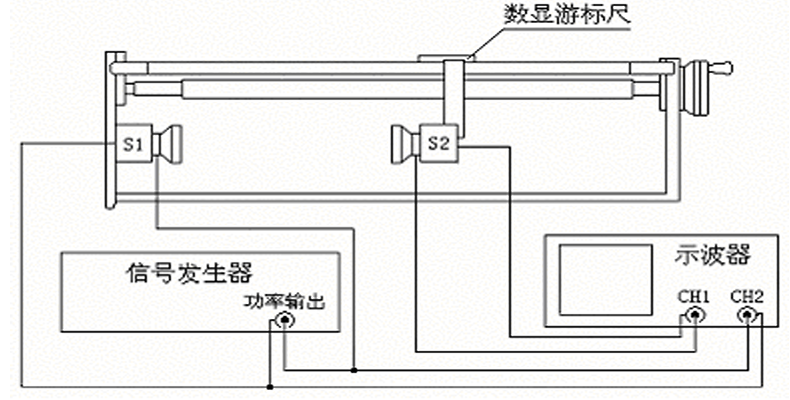
\includegraphics[width=0.4\textwidth]{驻波法.png} % 替换 "example-image" 为您的图片文件名
			\caption{实验装置}
			\label{fig:example}
		\end{figure}

	\section{实验原理}
		本实验通过测出声波频率$f$和波长$\lambda$,利用公式$v = f \cdot \lambda$ ,计算得出在该实验环境下的声速 。
		
		\subsection{计算实验环境(26.1°C,湿度26.8\%)下的理论声速}
		声波在空气中的传播速度与声波的频率是无关的,而只取决于空气本身的性质。声速的理论值可通过下式计算:
			\begin{equation}
				v = \sqrt{\frac{\gamma RT}{\mu}}
			\end{equation}
			式中 $\gamma$ 为空气定压比热容与定体比热容之比,$R$ 为普适气体常量,$\mu$ 为气体的摩尔质量,$T$ 为热力学温度。在 $0^\circ \text{C}$ 时,声速 $v_0 = 331.45 \, \mathrm{m/s}$。显然在 $t^\circ \text{C}$ 时的声速应为:
			\begin{equation}
				v_t = v_0 \sqrt{\frac{T}{273.15}} = v_0 \sqrt{1+\frac{t}{273.15}}
			\end{equation}

		\subsection{计算声波频率}
			实验中超声波是由交流电信号产生的,所以公式$v = f \cdot \lambda$ 中声波的频率f就是交流电信号的频率,由信号发生器中的频率显示可直接读出。
	
		\subsection{驻波法计算声波波长}
			如Figure 1所示,超声发射器 \( S_1 \) 接收信号后发射平面超声波,部分被超声接收器 \( S_2 \) 接收并转换为电信号输入示波器,部分反射回 \( S_1 \) 。发射波与反射波在 \( S_1 \) 和 \( S_2 \) 之间叠加相干,形成驻波。\\
			由物理学定义及相关数学公式推导,可得在两波相遇处,合成的声波为$$x = (2A \cos 2\pi \frac{x}{\lambda}) \cos 2\pi f t$$
			上式表明,当移动 \( S_2 \),使 \( S_1 \) 与 \( S_2 \) 之间的距离 \( l \) 为半波长的整数倍时,即 $l = n \frac{\lambda}{2} (n = 1,2,3 \cdots)$ 示波器上可观察到信号幅度的极大值(或极小值)。相邻两极值点之间的距离为$\frac{\lambda}{2}$。
			
		\subsection{相位法计算声波波长}
			\begin{figure}[H]
			\centering
			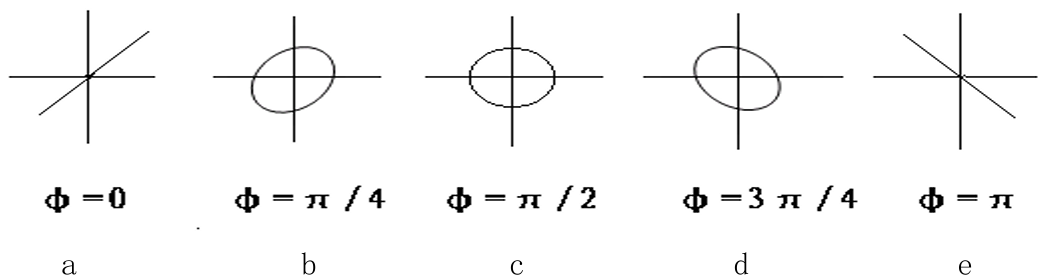
\includegraphics[width=0.75\textwidth]{李萨如图.png} % 替换 "example-image" 为您的图片文件名
			\caption{同频率互相垂直的谐振动合成的李萨如图形}
			\label{fig:example}
			\end{figure}
			发射器 \(S_1\) 发出的超声波为平面波,在传播方向上,相位相同或相差 \(2\pi\) 的整数倍,对应的距离 \(l\) 为波长的整数倍,即$l = n\lambda (n \text{ 为正整数})$
			为此,根据两个互相垂直的简谐振动的合成所得的李萨如图测定相位差。由于两端电信号频率相同,该图的形状由两信号的相位差 \(\Phi\) 决定。对 Figure 2 所示的图形的观测,即可确定相位差,从而确定声波的波长。


	\section{实验内容}
		\subsection{测量声速测定仪的共振频率}
		不断改变信号源所产生的频率,观察波形 2 峰值的变化。通过旋转鼓轮观察波形 2 的峰值,当旋转鼓轮前进或倒退,2 波形的最大峰值均减小,则此时为共振频率。
		\subsection{驻波法测声速}
		示波器采用 YT 模式,记录节点的位置,节点处振幅为零即声压最大,对应的振幅最大,通过旋转鼓轮观察波形 2 的峰值,当旋转鼓轮前进或倒退,2 波形的最大峰值均减小,则此目标为节点位置,记录此时的刻度,记为第一个节点,用同样的方法寻找下一个节点,直到第 12 个。
		\subsection{相位比较法测声速}
		示波器转换成 XY 模式,通过旋转鼓轮找直线图形,记录此时的刻度,依次记录 12 个相同形状的直线的位置。

	\section{数据记录}
		记录数据,输入excel制表计算

	\section{数据处理}
		\begin{figure}[H]
			\centering
			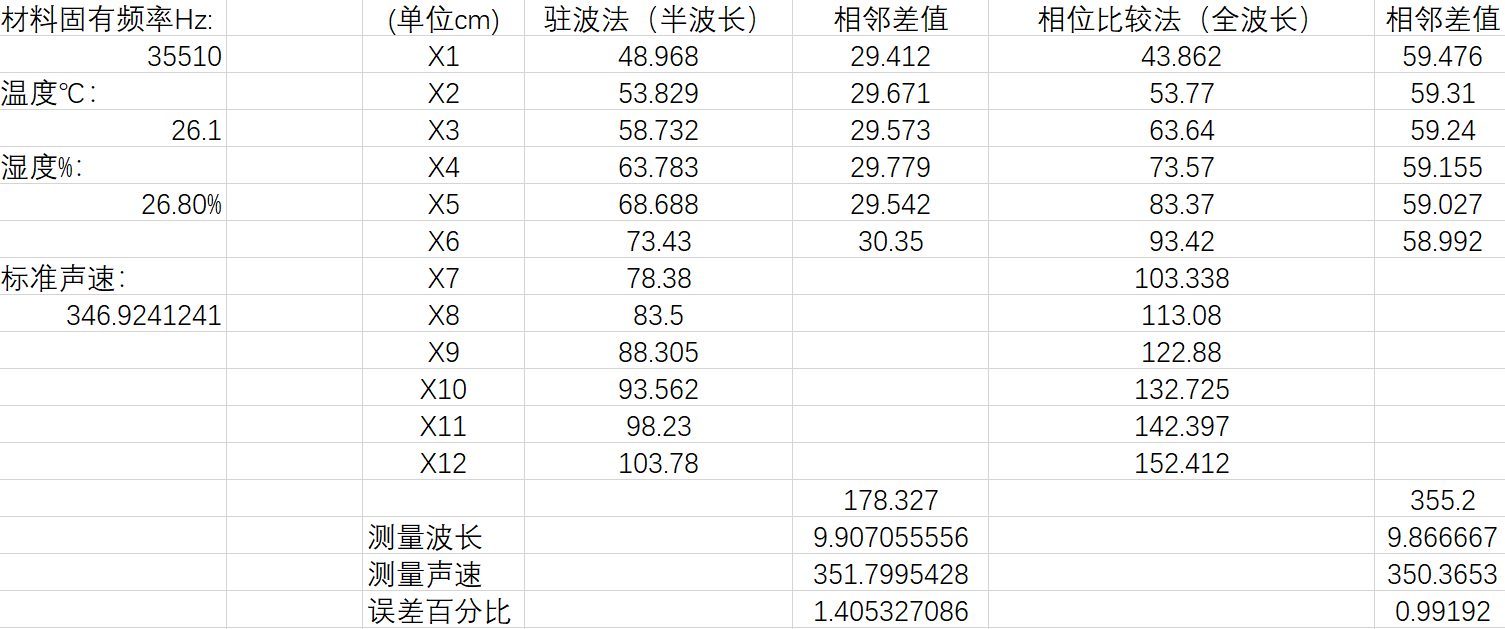
\includegraphics[width=0.75\textwidth]{数据.png} % 替换 "example-image" 为您的图片文件名
			\caption{实验数据}
			\label{fig:example}
		\end{figure}

		\subsection{参考声速(26.1°C,湿度26.8\%)}
			$v_{声} = v_0 \sqrt{1+\frac{t}{273.15}} = v_0 \sqrt{1+\frac{26.1}{273.15}} \approx 347 m/s  $
		\subsection{驻波法测声速}
			$\lambda_{1}=|(x_{7}-x_{1})+(x_{8}-x_{2})+(x_{9}-x_{3})+(x_{10}-x_{4})+(x_{11},-x_{5})+(x_{12}-x_{6})|\div6\div6\times 2 \approx 9.91 mm$
			$$v_{1} = f \cdot \lambda_{1} \approx 9.91*35.51 \approx 351.80 m/s$$
			$$相对误差\varepsilon_{1}=|v_1-v_{声}| \div v_{声} = |351.8-347| \div 347 \times 100 \% \approx 1.4\% $$
		\subsection{相位法测声速}
			$\lambda_{2}=|(x_{7}-x_{1})+(x_{8}-x_{2})+(x_{9}-x_{3})+(x_{10}-x_{4})+(x_{11},-x_{5})+(x_{12}-x_{6})|\div6\div6\times 2 \approx 9.87 mm$
			$$v_{2} = f \cdot \lambda_{2} \approx 9.87*35.51 \approx 350.37 m/s$$
			$$相对误差\varepsilon_{2}=|v_1-v_{声}| \div v_{声} = |350.37-347| \div 347 \times 100 \% \approx 0.99\% $$

		\subsection{(驻波法)不确定度计算}
		A类不确定度:
			$$\overline{\lambda}=  \frac{\lambda_{1} \times 6}{2} = 29.721 mm$$
			$$u_{\mathrm{A}} = \sqrt{\frac {\sum_{i=1}^{5}(\lambda_{i}-\overline{\lambda})^2}{6 \times 5}} = \sqrt{\frac{0.550391}{30}} \approx 0.1354 \approx 0.14 mm$$

		B类不确定度:
			$\quad \Delta_{\text{仪}} = 0.005 mm \quad \Delta_{\text{估}} = 0.001 mm $
			\[u_B=\sqrt{\Delta_{\text{估}}^2+\Delta_{\text{仪}}^2}/C=\frac{\sqrt{(0.005)^{2}+(0.001)^{2}}}{\sqrt{3}} \approx 0.0029 mm \]

		不确定度的合成:$(P=0.95)$
			
			对于重复测量次数为 12,则自由度为 \(12-1=11\)。根据分布表,在 95\% 置信水平下,覆盖系数为$t_{0.95} \approx 2.201$ ;\quad B类不确定度系数$k_{0.95}=1.96$
			$$u_{p}=\sqrt{(t_{0.95}u_{A})^{2}+(k_{0.95}u_{B})^{2}}=\sqrt{(2.201 \times 0.1354 )^{2}+(1.96\times0.0029)^{2}} \approx 0.30 mm$$

			谐振频率只有 B 类不确定度:
			频率的最小分度为 \(0.01\,\text{kHz}\),因此取$\Delta = 0.005\,\text{kHz}$.
			那么,
			\[
			u_B(f) = \frac{0.005}{\sqrt{3}} \approx 0.002887 \approx 0.0029\,\text{kHz} \Rightarrow u(f) =1.96 \times 0.002887 \approx 0.00566 \approx 0.0057\,\text{kHz}
			\]

			声速v的不确定度:
			\[
			\frac{U_{0.95}(V)}{V_1} = \sqrt{\left(\frac{U_{0.95}(V_1)}{V_1}\right)^2 + \left(\frac{U_{0.95}(f)}{f}\right)^2} = \sqrt{\left(\frac{0.30}{9.91}\right)^2 + \left(\frac{5.66}{3551.00}\right)^2} \approx 0.0303 \approx 0.030
			\]


			\[
			U_{0.95}(V) = 0.0303 \times 347.4 \approx 10.52 \approx 11 \, \text{m/s},\quad P = 0.95 
			\]

			\[
			V = V_1 \pm U_{0.95}(V) = 347 \pm 11 \, \text{m/s},\quad P = 0.95 
			\]


		误差分析:
		\begin{enumerate}
			\item 实验环境湿度为湿度26.8\%,但计算理论声速时未考虑
			\item 确定谐振频率时,肉眼可辨图像精度最低只能到0.01kHz
			\item 超声波多次反射,可能与原超声波叠加,造成误差
			\item 观察示波器中的李萨如图形是,不能精确地形成直线,导致位置确定的误差
		\end{enumerate}

	\section{问题思考}
		Q1:固定两换能器的距离改变频率,以求声速,是否可行?\\
		A1:理论可行——声速 $v$ 满足 $v = \lambda \cdot f$。若换能器间距离 $L$ 不变,通过改变频率 $f$,可以寻找使声波在这段距离上形成稳定干涉或共振(如驻波)的条件,从而推算出波长 $\lambda$,再由公式 $v = \lambda \cdot f$ 计算出声速 $v$

		Q2:各种气体中的声速是否相同,为什么?\\
		A2:\textbf{基本公式:} 理想气体中,声速可近似:
		\[
		v = \sqrt{\frac{\gamma R T}{M}}
		\]
		其中 \(\gamma\) 是定压定容比热容之比,\(R\) 是气体常量,\(T\) 是热力学温度,\(M\) 是气体的摩尔质量。
		不同气体具有不同的分子量 \(M\) 和比热容比 \(\gamma\);即使在相同温度下,声速也会不同。\\
		故,不同气体中的声速并不相同,根本原因在于气体的分子量、比热容比等物性参数不同,导致其在各种气体中具有不同的声速。
	
	\section{实验结论}
		本实验通过实验仪器,通过驻波法和干涉法测定了实验环境(26.1°C,湿度26.8\%)下的声速,并计算出了理论声速。
		分别为: 
		\paragraph{理论声速} $v_{声} = v_0 \sqrt{1+\frac{t}{273.15}} = v_0 \sqrt{1+\frac{26.1}{273.15}} \approx 347 m/s  $
		\paragraph{驻波法}	$V = V_1 \pm U_{0.95}(V) = 347 \pm 11 \, \text{m/s}, P = 0.95 \quad \text{误差百分比为}1.4\%$
		\paragraph{干涉法}	$v_{2} \approx 350.37 m/s$ \quad 误差百分比为0.99\%

\end{document}
